\subsection{Un nuevo modelo para Smart Campus}

Dado que no hay una alternativa que se adapte completamente a las necesidades del proyecto, se tuvo que definir una notación propia, la cual permita modelar las arquitecturas a nivel de aplicación bajo el contexto de un Smart Campus, tomando en cuenta los criterios definidos como guía para el desarrollo.

Primeramente, fue necesario definir un metamodelo que permitiera establecer la manera en la que se ven estas arquitecturas. Para ello, y partiendo de la implementación a realizar, se apoyó parcialmente en el modelo establecido por \citeA[p. 63]{msc_henry_2022}. 

\begin{figure}[H]
    \centering
    \caption{Versión 2 del modelo concepto planteado por \protect\citeauthor{msc_henry_2022}}
    \label{fig:henrymodelo}
    \vspace{2mm}

    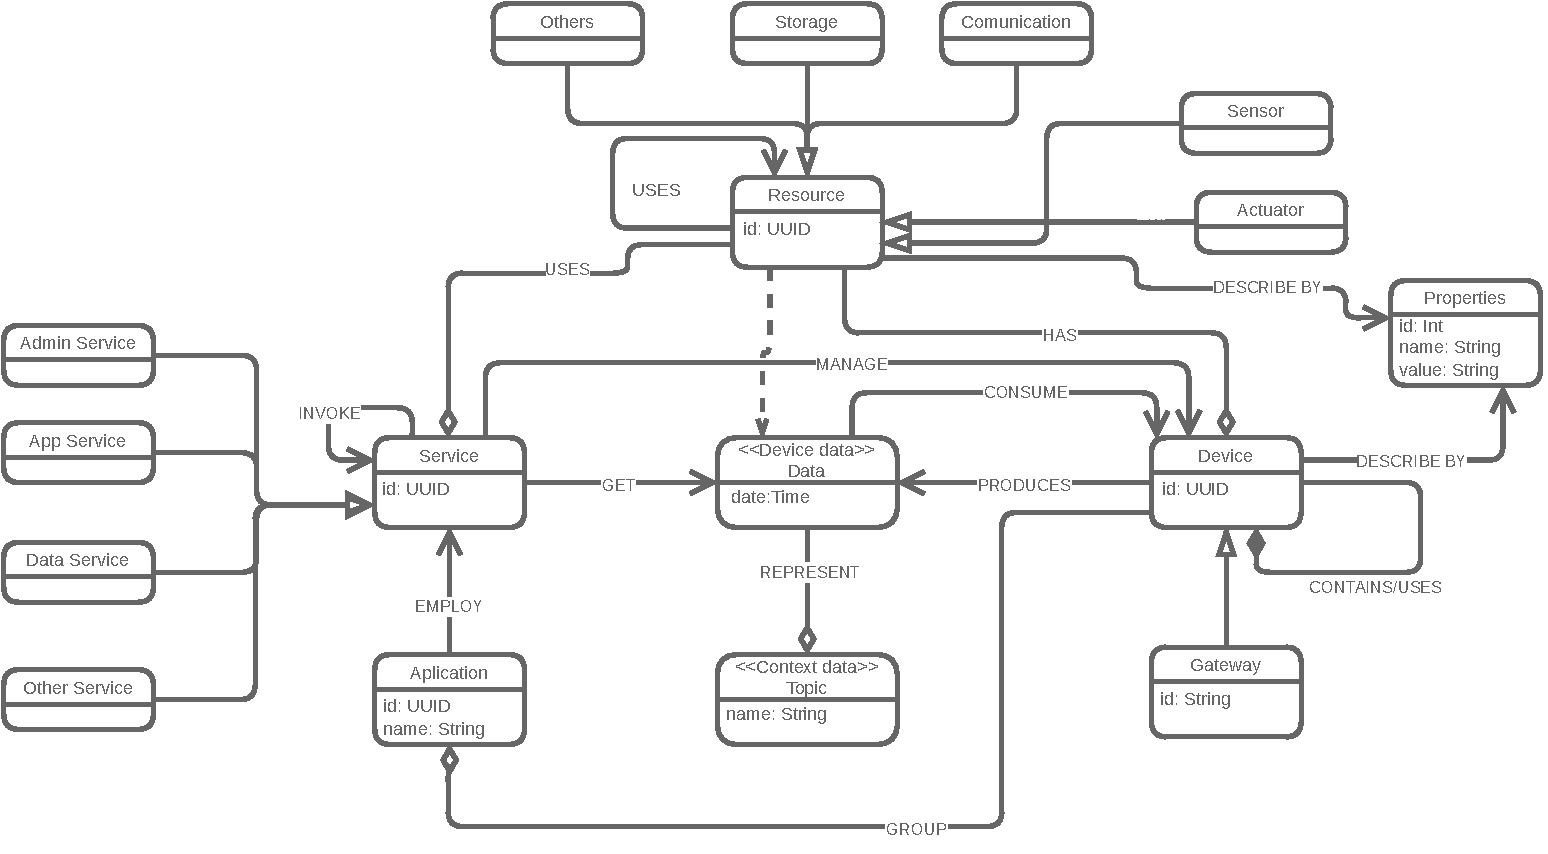
\includegraphics[width=\linewidth]{images/HenryModelo.pdf}
\end{figure}

Basarse en el modelo de la figura \ref{fig:henrymodelo}, da la capacidad de describir a un nivel técnico un sistema IoT. Ahora, aunque se podría usar para el desarrollo del proyecto, fue necesario modificarlo, con el fin de acercarnos más hacia la descripción de un sistema IoT a nivel de aplicación. 

El primer paso fue establecer el contexto de los dispositivos. Esto específicamente se refiere al criterio \textit{C2} de la tabla \ref{tab:criterios}, en donde, dada la necesidad de establecer la ubicación geográfica en algunas de las aplicaciones de los Smart Campus, era necesario poder describir los lugares pertenecientes a la aplicación.

Así mismo, se cubre el criterio \textit{C3} cambiando las propiedades del dispositivos de una clase, externa a los dispositivos; a un atributo, interno, el cual le permite a los componentes manejar su propia información en cuanto a los datos que estos manejan. Estas propiedades pueden referirse a las entradas que tienen, en el caso de ser actuadores o procesadores de la información; o a los valores que reportan al sistema en el caso de ser sensores.

Ahora, algo importante a tener en cuenta, es la manera en la que se están reportando los datos desde los sensores hacia Smart Campus UIS. Esto se debe a la necesidad de tener en cuenta los datos a los cuales tenemos realmente acceso desde cada uno de los dispositivos.

Cada uno de los dispositivos de Smart Campus, reporta un `JSON` similar al presente en la figura \ref{fig:jsonSCU}. Este mensaje contiene información que permite identificar al dispositivo, gracias al \textit{UUID}; al igual que el momento y los datos que este reporta.

\begin{figure}[H]
    \centering
    \caption{Mensaje JSON enviado por los dispositivos en Smart Campus UIS }
    \cite{SmartCampusGithub}
    \label{fig:jsonSCU}
    \begin{tabular}{c}
        \setstretch{1}
        \small
        \begin{lstlisting}[language=Json]
            {   
            "deviceUUID": "1",
            "topic": "temperatura",
            "timeStamp": "06-01-2024 10:39:02",
            "values": {
                "temperature": 10.0,
                "co2": 15.0,
                "location": "AP2" 
            },
            "status": "OK",
            "alert": false  
            }
        \end{lstlisting}
    \end{tabular}
\end{figure}

Es importante destacar que, aunque contamos con suficiente información para identificar los dispositivos, en estos mensajes no está presenta información crucial para el mapeo físico de los dispositivos. Por lo tanto, será necesario proporcionar manualmente estos datos durante la etapa de adaptación para llevar a cabo los ajustes necesarios en la arquitectura.

Partiendo de esto, se desarrolló el UML presente en la figura \ref{fig:metamodelo}. La base de este es la aplicación (\textit{\texttt{Application}}). Este contiene, a partir de una ubicación raíz, todas las demás locaciones (\textit{\texttt{location}}) pertinentes para el correcto funcionamiento de esta.

\begin{figure}[ht]
    \centering1
    \caption{Versión 1 del metamodelo planteado para SCampusADL}
    \label{fig:metamodelo}
    \vspace{2mm}
    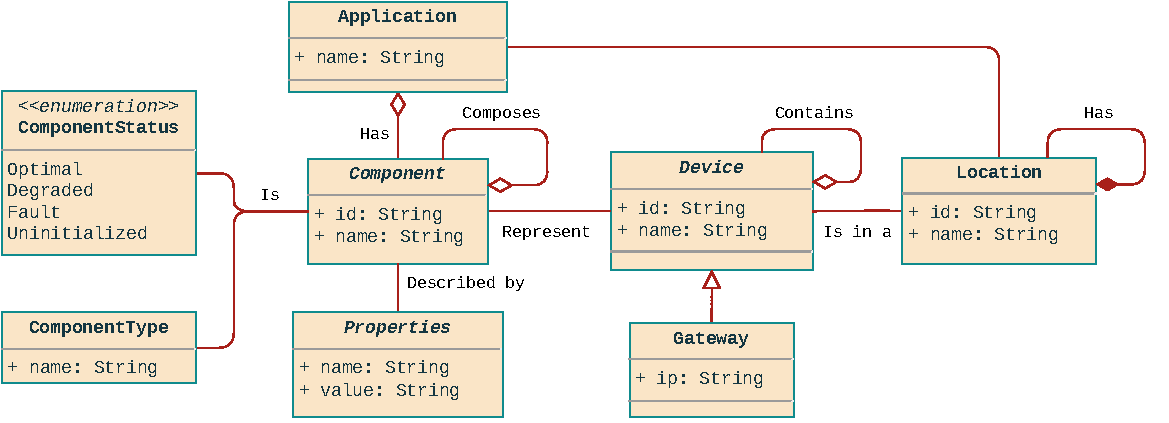
\includegraphics[width=\linewidth]{images/Metamodel B.pdf}
\end{figure}

Las locaciones, tienen una serie de requerimientos de datos (\texttt{\textit{DataRequirements}}), las cuales son las representaciones lógicas, o de software, de las necesidades de la aplicación. Estos pueden ser de 2 tipos: requeridos, que son aquellos con los cuales de no tenerlos, la aplicación no podría funcionar correctamente; y los opcionales, los cuales, aunque buenos de tener, no impiden el funcionamiento.

Cada uno de estos requerimientos de datos, contiene la cantidad de dispositivos, y a su vez datos, requeridos por la locación, al igual que el tipo de datos esperado (\textit{\texttt{IoTOutput}}), y el que el tiempo máximo permitido entre reportes de datos. 

Los requerimientos de datos, llevan un registro de los componentes (\textit{\texttt{Component}}) que han reportado datos en la locación. Esto permite evaluar cada uno de estos, y en la misma medida, determinar el estado (\textit{\texttt{Status}}) de cada una de las locaciones registradas en la aplicación. Estos estados buscan describir qué tan diferente es lo observado de lo esperado al igual que la validez de cada una de las partes. 

Ahora, las aplicaciones, en cierta medida, con el fin de llevar el registro de los datos enviados, consumen el mensaje JSON visto en la figura \ref{fig:jsonSCU}. Este ha sido deserializado y mapeado en \textit{\texttt{SCMessage}}. De esta manera, se podrá trabajar de manera sencilla en el procesamiento y actualización del estado de las aplicaciones.

De este modelo, se desarrolló e implementó una librería, apodada \textit{StarDuck}\footnote{El código fuente de la librería puede encontrarse en \url{https://github.com/ChipDepot/StarDuck}, y su respectivo paquete en crates.io, en \url{https://crates.io/crates/starduck}.}. Esta librería contiene todas las estructuras de datos definidas en el modelo, las cuales serán usadas por el resto de los servicios y aplicativos necesarios para la declaración, evaluación y adaptación de las arquitecturas de software en el proyecto. 
